\chapter{Proposta de Trabalho}
\label{chap:proposta}

Neste capítulo é discutido um plano de trabalho que será elaborado
durante o período após a qualificação, e resultados esperados.
Este trabalho tem o objetivo de trazer duas contribuições:
\begin{enumerate}
    \item Uma opção no compilador GCC para que ele seja
capaz de compilar um único arquivo em paralelo sem utilizar a
estrutura do LTO. Isso é útil para desenvolvedores que trabalham
desenvolvendo grandes softwares iterativamente, pois deve minimizar
gargalos gerados por arquivos grandes e cobrir os casos onde o LTO gerou
binário menos eficiente que o processo clássico de compilação, fornecendo assim
uma alternativa ao LTO.
Essa tese se concentra em paralelizar os passos de otimização Intra Procedural
a nível de funções.

    \item Uma revisão sobre o que pode ser feito para acelerar o
processo clássico de compilação em máquinas \textit{manycore}, através
de paralelismo, e quais problemas devem ser atacados em trabalhos futuros.
Espera-se utilizar os resultados do item 1.
\end{enumerate}


\section{Paralelização do GCC com \textit{threads}}

Nesta subseção é apresentado o estado atual do projeto de paralelização
do GCC com \textit{threads}. O GCC foi escolhido como candidato para
paralelização pois (1) a comunidade demonstrou grande interesse no projeto,
conforme discutido na Seção 1, e (2) O autor desta tese ter alguma
familiaridade com o projeto, já tendo contribuído com este. Sendo assim,
utilizar outro compilador como o Clang para implementar o projeto demandaria
estudos sobre a estrutura do projeto e convencer parte da comunidade de que
o trabalho trás alguma vantagem ao projeto. Por outro lado, implementar um
novo compilador não é uma alternativa viável dado que um dos maiores gargalos
na compilação é o otimizador, peça que não seria possível implementar em
dois anos algo tão poderoso como o GCC ou o Clang.

Como atestado por \cite{PR84402}, há um gargalo de paralelismo dentro do
próprio GCC por conta de arquivos grandes, e \cite{mailgcc} também
relatou um gargalo em outro projeto interno. Uma das soluções para este
problema é melhorar o paralelismo dentro do GCC, tornando possível fazer
com que a compilação utilize mais núcleos de processamento.

Nesta discussão, foi proposto uma maneira de visualizar o problema de
paralelismo através de um gráfico gerado por dados de um GNU Make modificado.
Como a alteração no Make é razoavelmente complicada e o \textit{script} proposto
havia sérios problemas de estabilidade, foi desenvolvido uma outra maneira
de replicar os resultados.

Como desenvolvido e disponibilizado publicamente por \cite{gcctimer}, essa
ferramenta é capaz de coletar e exibir dados referente ao tempo de compilação
de cada arquivo no GCC, incluindo os testes gerados pelo GNU Autotools.
A ferramenta funciona da seguinte forma: há um programa escrito em C chamado
\texttt{cc\_wrapper} que encapsula o compilador C e C++ do ambiente, no caso o 
GCC e o G++. O caminho para estes compiladores são passados como um parâmetro
da compilação do \textit{cc\_wrapper} de maneira que os binários gerados os
simulem. Em seguida o programa abre um novo processo através do \texttt{fork()},
chamando o GCC/G++ com os parâmetros passados a ele sem alterações. O processo
inicia a coleta do tempo, busca pelo nome do arquivo objeto a ser gerado, e
aguarda o GCC chamado terminar. Essa busca foi codificada de maneira a ser
muito eficiente, tento um pior caso $O(n)$ com uma constante muito baixa,
onde $n$ é o número de parâmetros passados ao GCC. Em seguida, o programa
escreve o tempo de início, tempo de fim, e o nome do arquivo em um arquivo
de texto. Houve um cuidado para que não haja mistura de linhas
no arquivo por razão de escrita simultânea no arquivo.

Em seguida, foi codificado um programa em \textit{Python} para análise dos
resultados. Esse programa é responsável por gerar os gráficos conforme
mostrado na Figura \ref{fig:analysis_classical}. Em um dos eixos há o 
tempo de execução, no outro há
o trabalho do Makefile. Para construir tal gráfico é utilizado a técnica
de coloração em grafos de intervalos, que pode ser resolvido otimamente
em $O(n \log n)$, onde $n$ é o número de arquivos, embora o algoritmo
implementado seja $O(n^2)$.


\begin{figure}[ht]
 \centering
 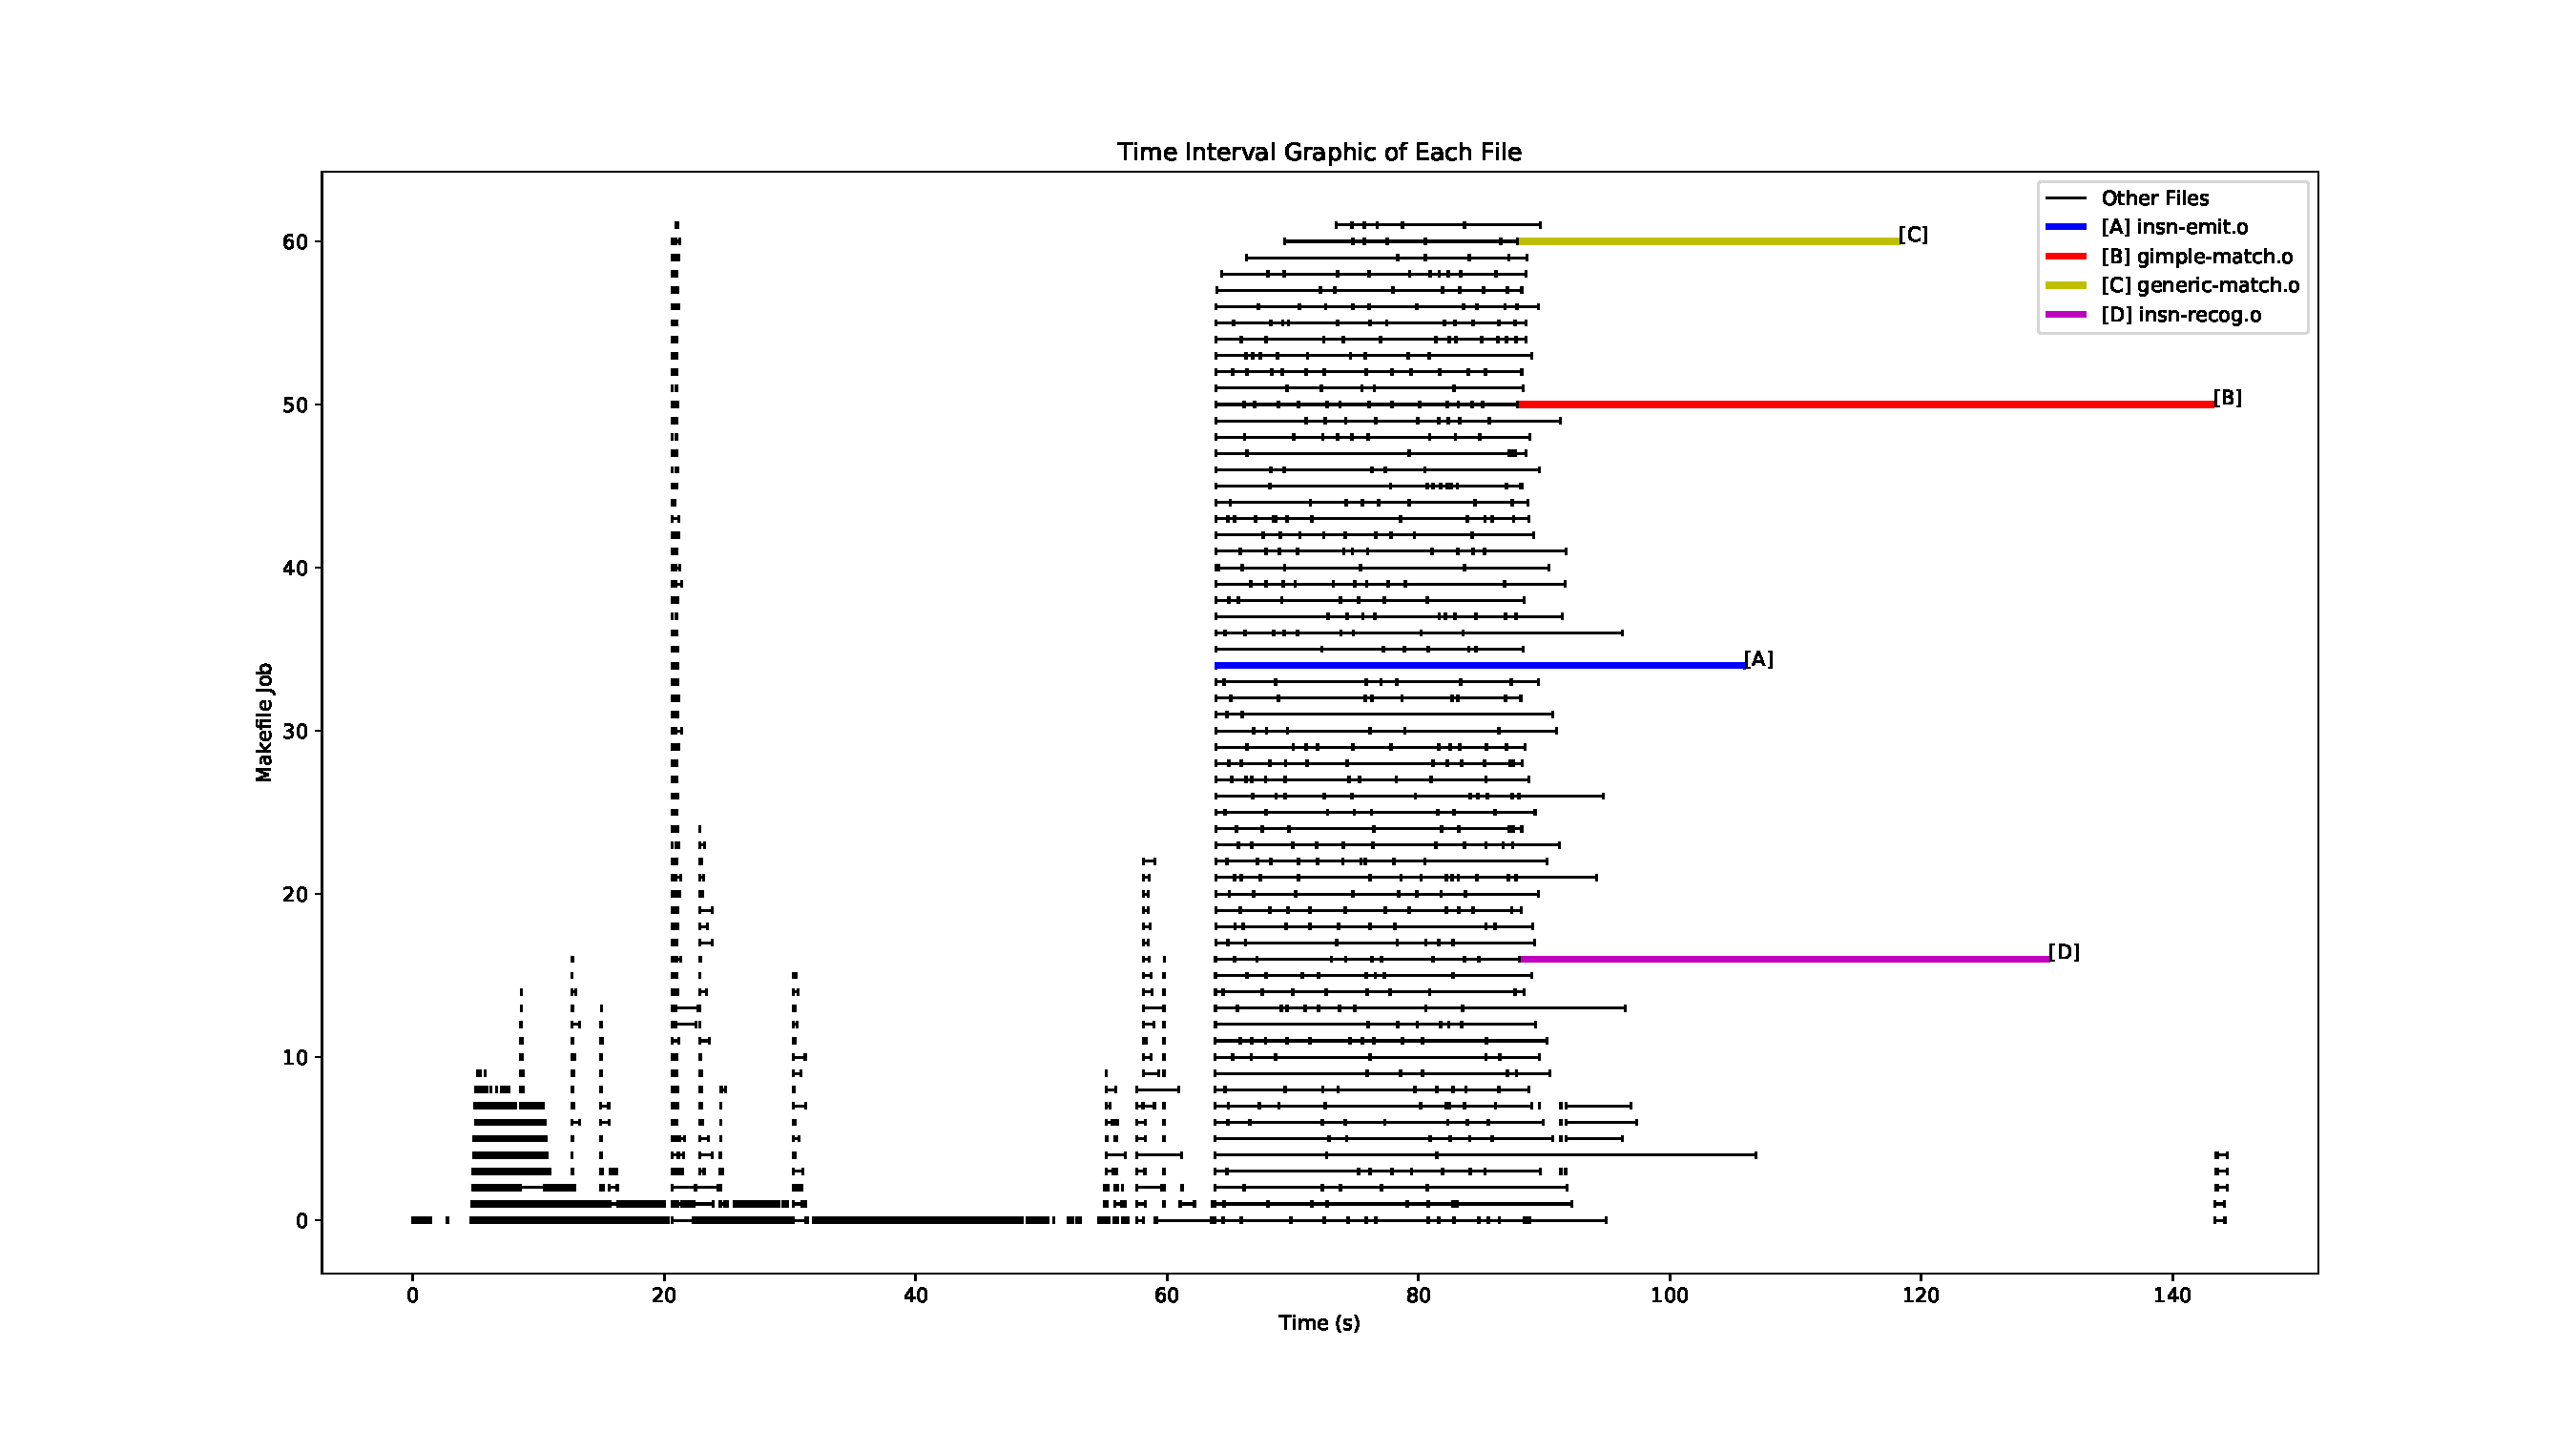
\includegraphics[scale=0.6, angle=-90]{gcc_timer_classic.pdf}
 \caption{Tempo corrido na compilação do GCC em um processador de 64 núcleos. Sem \textit{Bootstrap}}
 \label{fig:analysis_classical}
\end{figure}

%%%%%%% Cronograma %%%%%%%

\begin{figure}
  \centering

  \begin{ganttchart}{2017-11}{2018-5}
    \gantttitlecalendar{year,month=shortname} \ganttnewline

    \ganttgroup[progress=45]{Experimento}{2017-11}{2018-2} \ganttnewline
    \ganttbar[progress=100]{
      Preparação\ganttalignnewline
      (compra de insumos)
      }{2017-11}{2017-12} \ganttnewline
    \ganttbar[progress=30]{Execução}{2017-12}{2018-1} \ganttnewline
    \ganttbar[progress=0]{Análise}{2017-12}{2018-2} \ganttnewline

    \ganttgroup[progress=0]{Artigo}{2018-1}{2018-4} \ganttnewline
    \ganttbar[progress=0]{Escrita}{2018-1}{2018-3} \ganttnewline
    \ganttbar[progress=0]{Revisão}{2018-3}{2018-4} \ganttnewline

    \ganttmilestone{Submissão}{2018-4}
  \end{ganttchart}

  \caption{Exemplo de cronograma.\label{fig:gantt}}
\end{figure}

%%%%%
